%=========================================================================%
%    10TH INTERNATIONAL SYMPOSIUM ON PARTICLE IMAGE VELOCIMETRY - PIV13
%
%    prepared by 	Callum Atkinson - 26/04/2008, Julio Soria - 29.09.2008, Jun Sakakibara - 12.18.2009
%    modified by	Christian Poelma - 9/10/2012
%
%    Format: LaTeX2e.
%=========================================================================%
\documentclass{piv13-abstract}
\usepackage[pdftex]{graphicx}
%\usepackage[none]{hyphenat}	% disable hyphenation of text in columns
\usepackage{subfigure}
\usepackage{bm}
\usepackage[numbers]{natbib}
\usepackage{placeins}

\usepackage{color}
\newcommand{\hilight}[1]{\colorbox{yellow}{#1}}
\newcommand{\unit}[1]{\ensuremath{\, \mathrm{\hspace{0.5mm}#1}}}
\newcommand{\vect}[1]{\vec{#1}}
\newcommand{\matr}[1]{\bm{#1}}
\newcommand{\figLabel}{Fig. }
\newcommand{\figsLabel}{Figs. }
\newcommand{\eqLabel}{Eq. }
\newcommand{\eqsLabel}{Eqs. }


\begin{document}

\title{Flow measurements near the boundary of a finite turbulent patch in stable stratification}

\author{Zachary J. Taylor$^1$, Roi Gurka$^2$, Peter J. Diamessis$^3$, and Alex Liberzon$^1$}
\affiliation{$^1$ School of Mechanical Engineering, Tel Aviv University, Tel Aviv, Israel,
zacharyt@post.tau.ac.il\\
		\vspace{2pt}
	     $^2$ Department of Mechanical Engineering, Ben-Gurion University, Beer-Sheva, Israel\\
         \vspace{2pt}
         $^3$ School of Civil and Environmental Engineering, Cornell University, Ithaca, NY, USA\\
}

\maketitle

\begin{abstract}

Turbulent patches are a common feature in the ocean, yet many questions remain concerning the mixing characteristics of these patches in stably stratified environments. A three-dimensional, finite patch of turbulence is formed by an oscillating grid in both fresh water and an index-of-refraction matched stably stratified solution. Optical measurements including synchronized particle image velocimetry and planar laser induced fluorescence have been performed to capture the life cycle of the patch from its initial growth until it reaches critical height followed by its eventual collapse. The simultaneous capture of density and velocity allows for an assessment of both the density interface of the patch and the turbulent/non-turbulent interface. The experimental data suggest that the density boundary becomes more diffuse as the grid-generated turbulence increases.

\end{abstract}

\section{INTRODUCTION}
\label{sec:intro}

One of the most fundamental features of ocean turbulence is diapycnal (i.e., across lines of constant density) mixing which appears to be three-dimensional \cite{bookThorpe2005}. The ocean pycnocline, occurring below the mixed surface layer, is the area where the stratification is stable and the density gradient, $\partial\rho/\partial z$, is largest.  From various experiments within the ocean pycnolcine, it has been suggested that there are relatively localized regions of high-intensity turbulence with vertical scales on the order of \emph{O}(10 m) with larger horizontal scales \cite{Nasmyth1970}.  These observations have motivated the exploration of the characteristics and driving mechanisms of finite, three-dimensional turbulent ``patches'' in stably stratified environments. 

A simplified process for the growth and collapse of a turbulent patch is provided by Sundermeyer and Ledwell \cite{Sundermeyer2001} whose sketch is adapted here in \figLabel\ref{fig:thorpe}. The proposed process is also discussed by Thorpe \cite{bookThorpe2005} and Sundermeyer et al. \cite{Sundermeyer2005}. It is assumed that these patches of turbulence are formed by the breaking of internal waves \cite{Garrett1972,Garrett1979} which initially mixes a localized region, significantly deforming the isopycnal lines, until a patch of constant density is formed. The resulting pressure forces acting at the top and bottom of the patch, due to the ambient stratification, act to compress the patch in the vertical direction which forces its lateral spreading and intrusion into the surrounding fluid. 

\begin{figure}[ht]
\centering
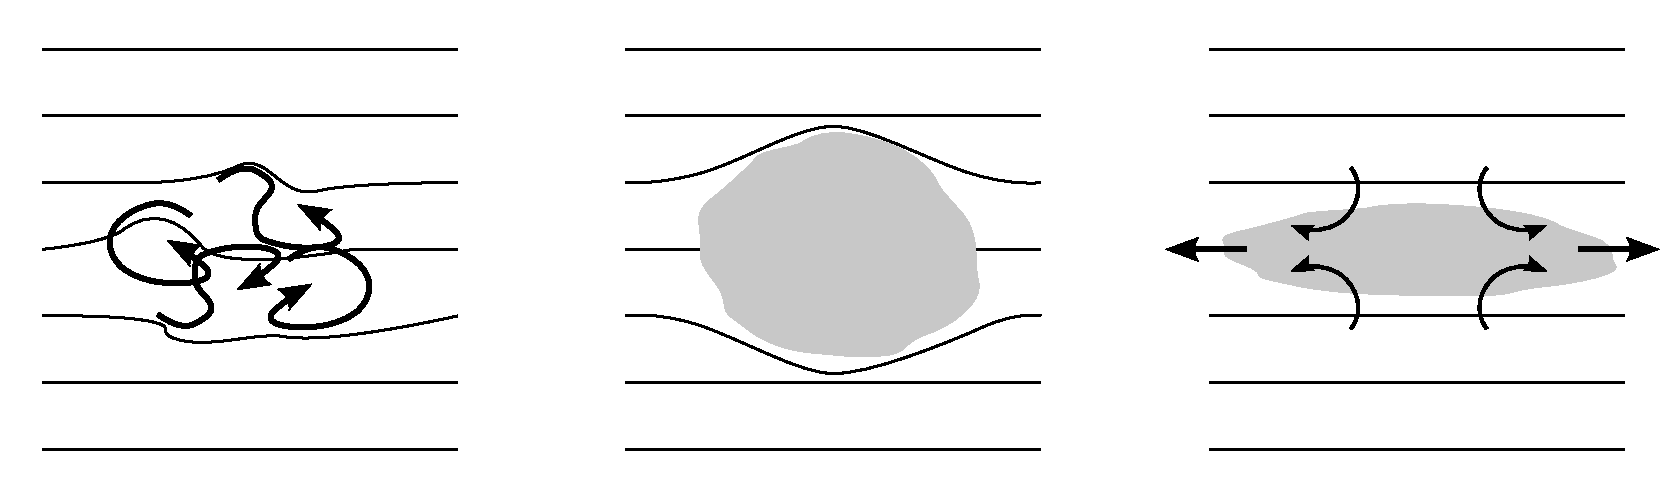
\includegraphics[width=0.7\textwidth]{figures/thorpesvg.pdf}
\caption{The horizontal lines represent isopycnal (constant density) lines which are initially mixed due to turbulence. The density within the patch becomes relatively homogeneous. Due to the background stratification, pressure forces act to restrict the growth of the patch in the vertical direction, and lateral intrusions are formed. \label{fig:thorpe}}
\end{figure}

In the current study, laboratory measurements are performed on a finite, three-dimensional turbulent patch in a stably stratified fluid. One of the first studies on a patch of turbulence in stable stratification was by Barenblatt and Moin \cite{Barenblatt1979}. They generated a patch by oscillating a grid vigorously inside of a cylinder so that the surrounding stratification was unaffected. Once the fluid inside the cylinder was sufficiently mixed, the grid and cylinder were removed and the evolution of the turbulence observed. As the patch collapsed vertically, a horizontal intrusion was formed. Likewise, a horizontal intrusion was observed in the earlier experiment by Wu \cite{Wu1969} who measured the evolution of an intrusion formed by the injection of a patch of fluid with uniform density into a stably stratified environment. The growth of a one-dimensional turbulent patch was studied by Fernando \cite{Fernando1988} by using a span-filling grid oscillating in the vertical direction of a linearly stratified fluid .  By continuously forcing the patch it was found that its growth was initially unaffected by the stratification.  However, the size of the patch reached a critical level and vertical growth was observed to cease.  Likewise, in the case of a two-dimensional patch with continuous forcing, de Silva and Fernando \cite{Silva1998} found that the patch spread horizontally, forming an intrusion, once its vertical growth was restricted at approximately the same time as the one-dimensional case. 

The suggestion of the simplified model in \figLabel\ref{fig:thorpe} is that there is a distinct boundary formed between the background density stratification and the homogeneous density within the patch. The data taken by de Silva and Fernando \cite{Silva1998} seem to support this notion with entrainment across the interface attributed mostly to return currents established by the horizontally spreading patch. However, measurements with detailed spatial resolutions are challenging and have not been performed on a finite patch of turbulence in stable stratification. Thus, the aim of the current study is to create a localized turbulent patch with varying intensities of turbulence in a stably stratified laboratory experiment. Simultaneous Particle Image Velocimetry and Planar Laser Induced Fluorescence measurements are used in order to gain insight into the dynamics near the density interface as the turbulence of the patch is varied. In addition, the life cycle of the patch is also studied through its growth, peak and collapse.

\section{EXPERIMENTAL SETUP}

\subsection{Density gradient}

The experiments are performed in a glass tank with a $20\times50\unit{cm^2}$ cross-section and a depth of 20 cm.  Experiments were carried out in two different solutions including a homogeneous (fresh water) solution and an index-of-refraction matched stratified solution of sugar water and Epsom salts \cite{McDougall1979} (see Section 2.3 for more details). The degree of stratification is given by the Brunt-V\"ais\"al\"a frequency, $N$, which is defined as
%
\begin{equation}
N^2=-\frac{g}{\rho_0}\frac{d\rho}{dz}
\label{eq:frequency}
\end{equation}
%
where $\rho_0$ is the density at mid-depth, and $d\rho/dz$ is the density gradient in the vertical direction. A stable linear density gradient (\figLabel\ref{fig:exp_schematic}) is established in the aquarium using the free-flow two-tank method \cite{Economidou2009}. The linear density profile is confirmed to correspond to a buoyancy frequency of $N=1\unit{rad\cdot s^{-1}}$ via a pycnometer by extracting small volumes of liquid at different depths.

\begin{figure}[ht]
\centering
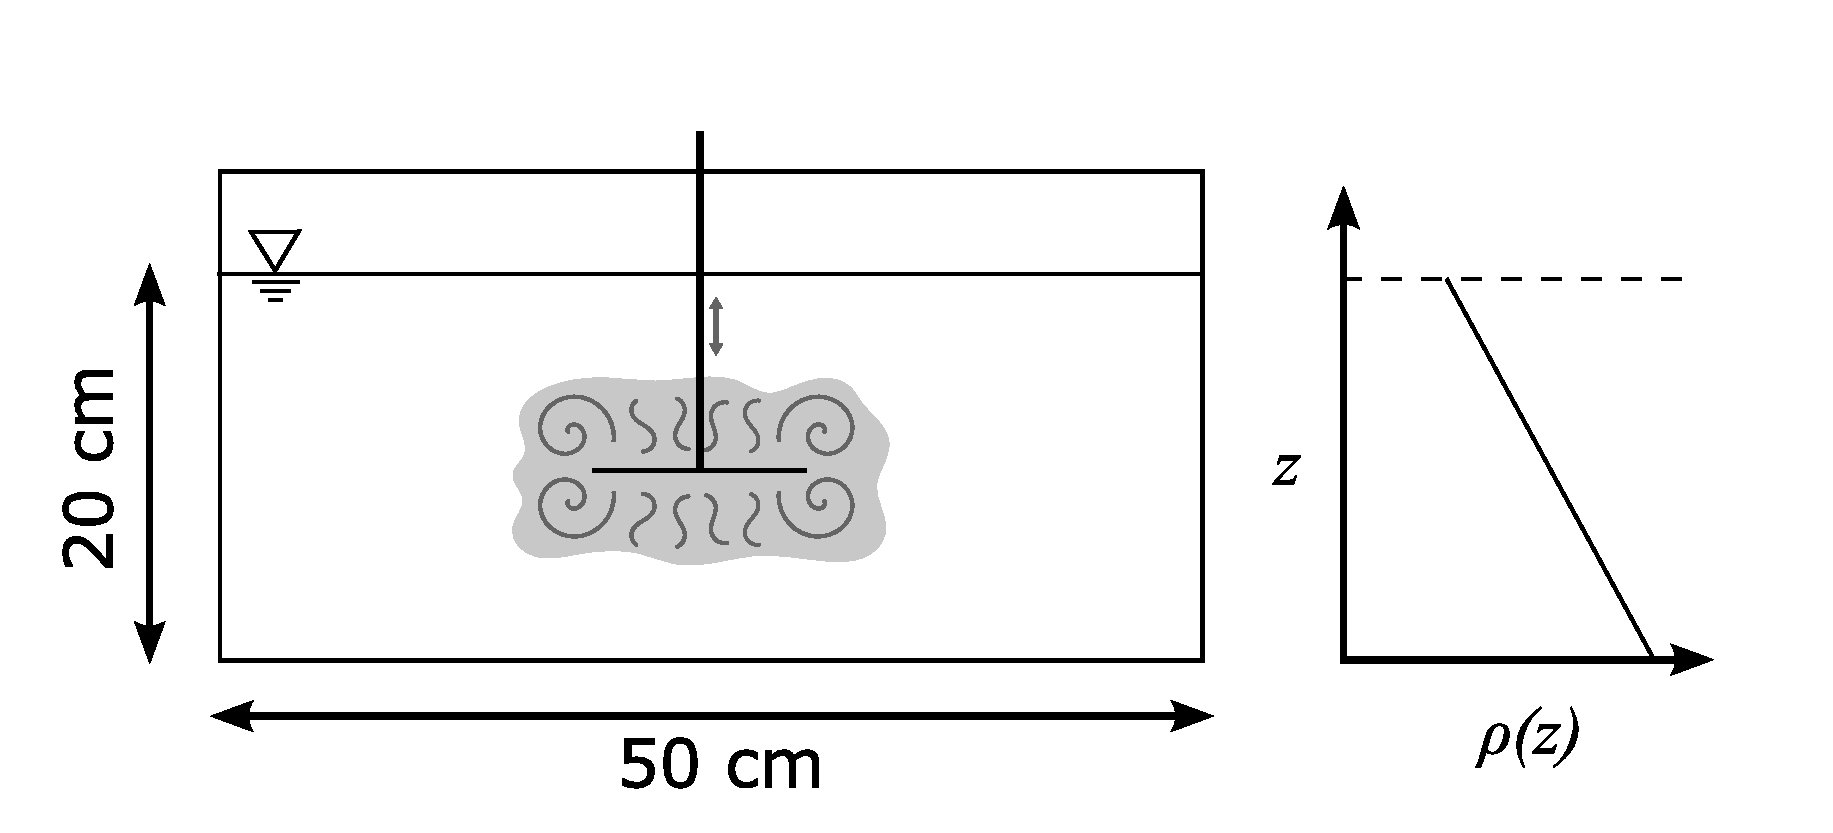
\includegraphics[width=0.65\textwidth]{figures/exp_schematic.pdf}
\caption{Illustration of the size of the aquarium, the density gradient, and the motion of the turbulence-generating grid. \label{fig:exp_schematic}}
\end{figure}

Once the aquarium was filled, the solution was allowed to settle in order to remove any discontinuities in the density gradient. The same solution could be used in multiple experiments with sufficient time allowed between experiments for the density gradient to return to the initial condition (see \figLabel\ref{fig:rho_profile}).

\subsection{Generating turbulence}

The patch is created using an oscillating grid located at the centre of the solution. The grid is $60\times60\unit{mm^2}$ with a bar size of 2 mm and a mesh size of 10 mm giving a solidity of 30.6\%. The oscillations are provided via a slide on a linear ball-bearing rail connected to a motor with an eccentric linkage. From the top of the stroke to the bottom of the stroke measures 1 cm. Over the first two seconds of the oscillations, the motor is provided a ramp input to minimize any impulse from the start-up procedure while the oscillations last for 8 seconds in total. The maximum frequency obtained after the initial ramp input ranges between 3 to 8 Hz in increments of 1 Hz.

In the case of stable stratification, the magnitude of the velocity fluctuations within the patch varied with the frequency of the oscillations and observed \emph{rms} values ranged between $0.5 < u^{\prime} < 1.5 \unit{cm\cdot s^{-1}}$.  Thus, a range of Froude numbers and Reynolds numbers (both scaled by the mesh size, $M$) are achieved, respectively:
\begin{equation}
Fr = \frac{u^{\prime}}{MN} = 0.5 - 1.5 
\end{equation}
\begin{equation}
Re = \frac{u^{\prime}M}{\nu} = 50 - 150
\end{equation}

\subsection{Matching index-of-refraction}
\label{sec:ior}

Obtaining a linear stable stratification using variations in salt concentration is a commonly used experimental technique (e.g., \cite{Fernando1988,Spedding1997,Silva1998}). However, when using optical methods there are legitimate concerns about the deviation of of the light path of the laser \cite{McDougall1979} in addition to the deviation of the light paths towards the camera \cite{Alahyari1994}. The solution in the present case follows the work of McDougall \cite{McDougall1979} who suggested the use of a sugar-water solution and an Epsom salt (MgS0$_4$) and water solution. The desired density difference of $20\unit{kg\cdot m^{-3}}$ between the bottom of the aquarium and the free surface was obtained with a maximum difference in the index-of-refraction of $\Delta n < 0.00001$, which compares favourably with previous studies \cite{Daviero2001}. This maximum difference in the index-of-refraction was obtained in each solution separately and when the two solutions are mixed \cite{McDougall1979}. 

\subsection{Particle Image Velocimetry}
\label{sec:PIV}

Two-dimensional, two-component Particle Image Velocimetry (PIV) measurements were performed in a vertical plane passing through the horizontal centre of the tank as shown in \figLabel\ref{fig:plif_piv_setup}. The PIV system used in this study is composed of a Nd:YAG laser with 120 mJ/pulse at a wavelength of 532 nm and a 11 MP double-exposure CCD camera with a 12-bit sensor. Fit to the camera was a 60 mm Nikkor lens, and the imaging set-up yielded a physical magnification of $56.2\unit{\mu m\cdot pixel^{-1}}$.

The PIV image pairs were processed using OpenPIV \cite{Taylor2010} with interrogation windows of $32\times32\unit{pixels^2}$ with 50\% overlap. Spurious vectors were identified first by a global filter and followed by a local median filter. The rejected vectors were replaced by interpolation using the local mean and the data were smoothed using a Gaussian filter.

PIV measurements were performed both in fresh water and in stable stratification. The fresh water experiments were used to determine the time between each image of an image pair, $\Delta t$. The value of $\Delta t$ was decreased as the frequency of the oscillations increased in order to obtain displacements of approximately 5 pixels.

External triggering was provided via a LabVIEW routine which initiated the motion of the grid and the first PIV image pair at the same time. In addition, the PIV measurements were synchronized with the PLIF measurements to obtain synchronized measurements of density and velocity.

\subsection{Planar laser induced fluorescence}
\label{sec:PLIF}

Planar laser induced fluorescence (PLIF) measurements were performed simultaneously with the PIV measurements using the setup shown in \figLabel\ref{fig:plif_piv_setup}. The goal of the PLIF measurements was to measure the density distribution over the entire imaging plane. Thus, Rhodamine 6G was added to the tank of heavier liquid (the Epsom salt solution) at a concentration of $50\unit{\mu g\cdot L^{-1}}$. It is then assumed that the density can be obtained indirectly through measurement of the concentration of the Rhodomaine 6G using PLIF. This technique has previously been used in the study of interfacial mixing in stratified environments \cite{Atsavapranee1997}, wave breaking \cite{Troy2005} and in stratified gravity currents \cite{Odier2009}. The assumption that the Rhodamine 6G follows the density field relies on the fact that the diffusivity of turbulence ($\kappa_T\approx u^{\prime}l=1 \unit{cm^2\cdot s^{-1}}$) is much greater than the molecular diffusivities of Rhodamine 6G ($\kappa_{R6G}=0.12\times 10^{-5}\unit{cm^2\cdot s^{-1}}$), Epsom salt ($\kappa_{MgS0_4}=0.61\times 10^{-5}\unit{cm^2\cdot s^{-1}}$), and sucrose ($\kappa_{sucrose}=0.45\times 10^{-5}\unit{cm^2\cdot s^{-1}}$). Thus, the Batchelor scale of the Epsom salt, based on the Kolmogorov length scale, $\eta\approx 0.2\unit{mm}$, and the Schmidt number, $Sc=\nu/\kappa$, was on the order of $\lambda_B=(\eta/Sc^{1/2})\approx O\left(10\unit{\mu m}\right)$, which is smaller than the size of 1 pixel ($56.2\unit{\mu m}$). When excited by the Nd:YAG laser at a wavelength of 532 nm, the Rhodamine 6G emits light at 555 nm; thus, a bandpass filter (Newport 20BPF10-550) with an admittance band of $550\pm10\unit{nm}$ was fitted to the camera. The camera used for the PLIF measurements was an additional 11 MP, 12-bit camera identical to that used for the PIV measurements with a 60 mm Nikkor lens and the aperture set to $f/2.8$.

\begin{figure}[h]
\centering
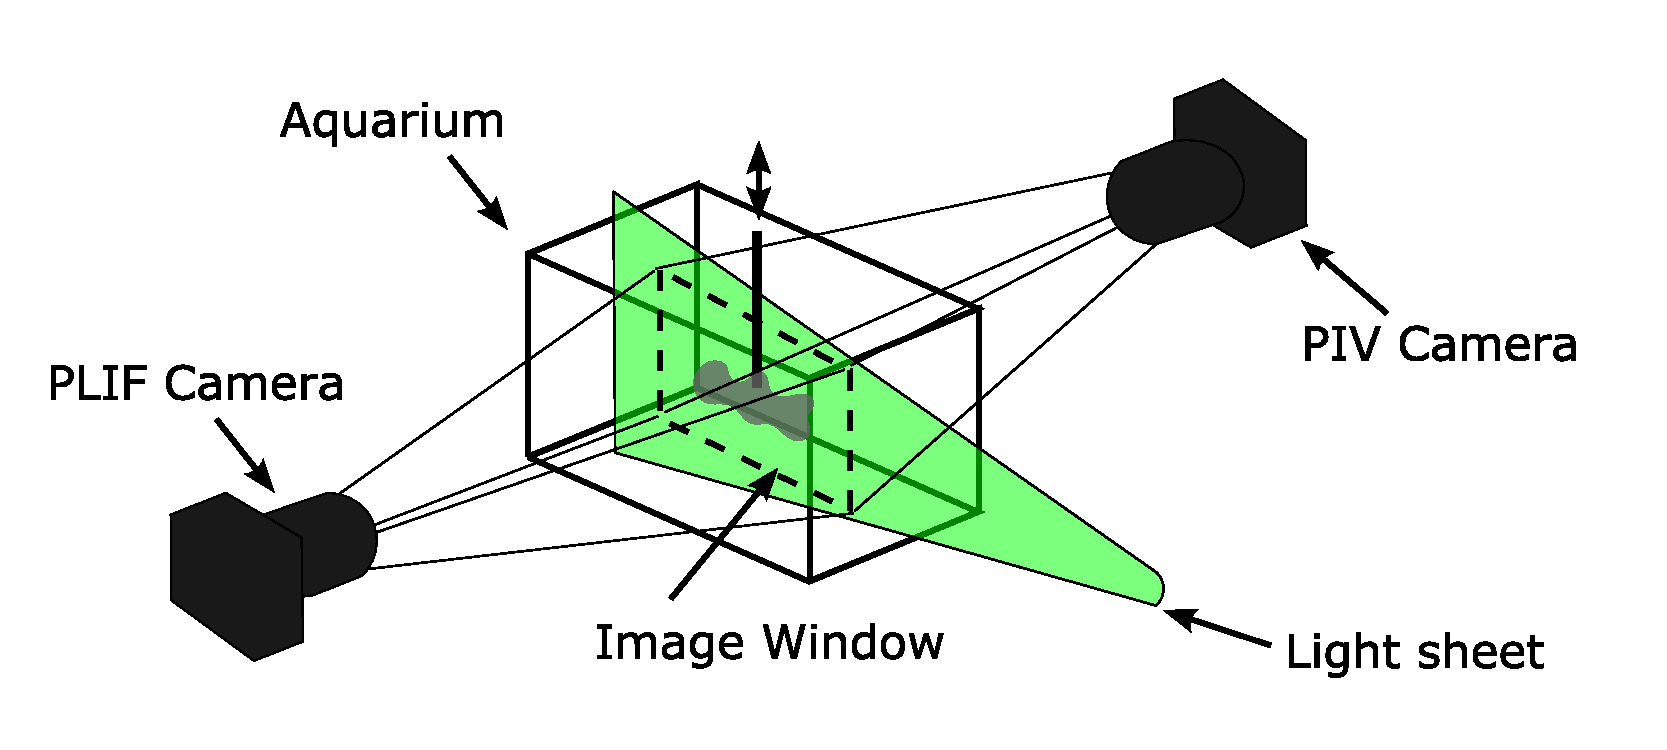
\includegraphics[width=0.6\textwidth]{figures/plif_piv.pdf}
\caption{Illustration demonstrating the position of the PIV and PLIF cameras and the light sheet orientation with respect to the turbulent patch. \label{fig:plif_piv_setup}}
\end{figure}

The calibration of the PLIF data was performed using five different uniform concentrations of Rhodamine 6G in the aquarium and a homogeneous mixture of Epsom salts, sucrose and water to replicate the experimental conditions as closely as possible. The concentration field was calibrated similarly to the method described in \cite{Crimaldi2008}. The pixel-by-pixel, concentration-independent, calibration coefficient, $\alpha\left[i,j\right]$ was obtained using an average of the five different uniform calibration concentration fields
%
\begin{equation}
\alpha\left[i,j\right] = \frac{1}{N_c}\sum_{c}\frac{I\left[i,j\right] - B\left[i,j\right]}{a\left(r,\theta\right)C\left[i,j\right]}.
\end{equation} 
%
The variation of $\alpha$ was typically below 2\% across all five separate calibrations. As shown in \figLabel\ref{fig:plif_piv_setup}, the center of the laser sheet passed through the aquarium travelling in the horizontal direction; therefore, it was necessary to calculate the concentration in a step-wise manner from one side of the image, $r_0$, to the other following the light beam paths of the laser sheet. The horizontal distance between the imaging plane and the entrance of the aquarium was 13.75 cm and the background gradient of the concentration was assumed for this section for which no image data were available. The attenuation of the laser was assumed negligible over the distance of air it travelled. In the imaging plane, the attenuation coefficient was computed as follows,
\begin{equation}
a(r,\theta) = \exp\left[-\epsilon\int_{r_0}^r C\left(r^{\prime},\theta\right)dr^{\prime}\right]
\end{equation}
%
where $\epsilon$ is the absorption coefficient.  The value of the absorption coefficient is $\epsilon = 1.1\times10^5\unit{\left(cm\cdot M\right)^{-1}}$ for Rhodamine 6G \cite{Ferrier1993}, and this value is assumed constant for concentrations below $50\unit{\mu g\cdot L^{-1}}$, which was the maximum concentration used in the current study.

\begin{figure}[ht]
\centering
\subfigure[]{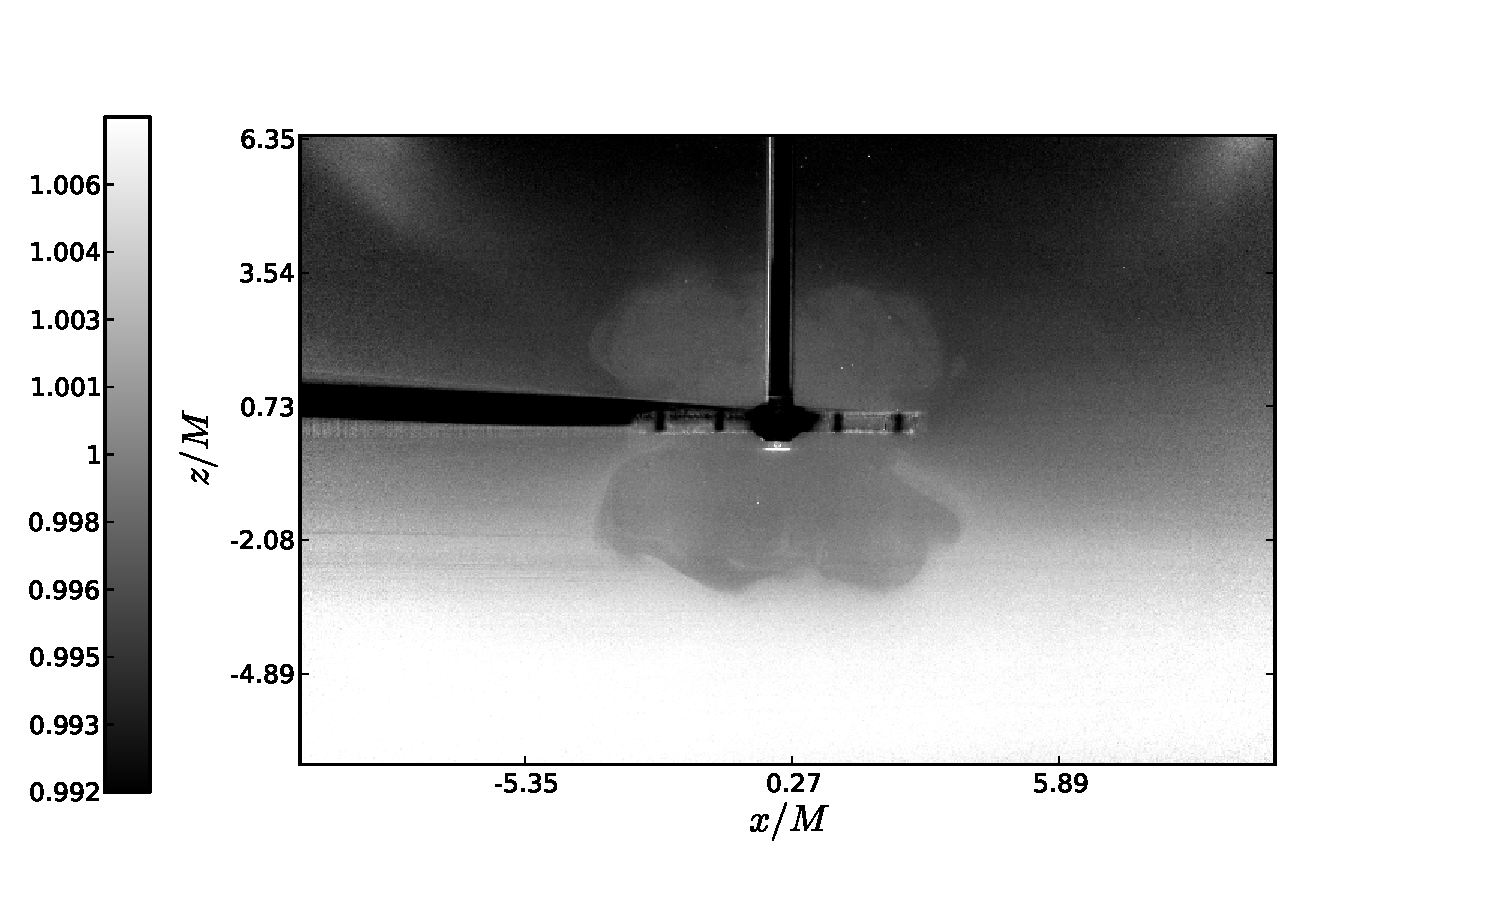
\includegraphics[width=0.45\textwidth]{figures/plifDemo.pdf}\label{fig:pivPlifDemo-plif}}
\subfigure[]{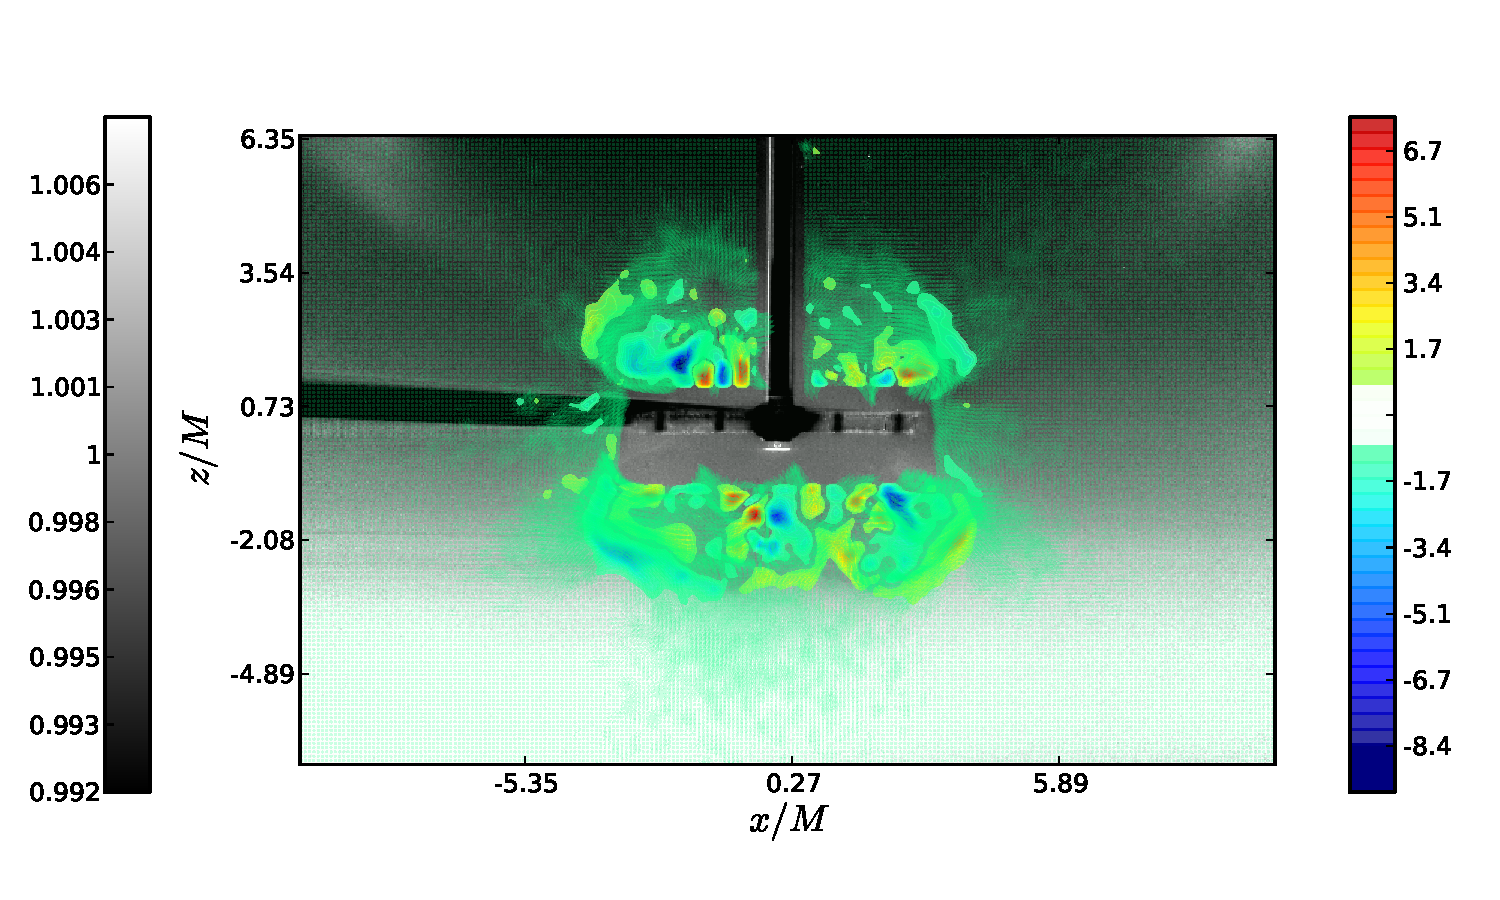
\includegraphics[width=0.45\textwidth]{figures/pivPlifDemo.pdf}\label{fig:pivPlifDemo-both}}
\caption{An example of the synchronized PIV/PLIF measurements with a PLIF capture shown by itself in \subref{fig:pivPlifDemo-plif}. The density values are indicated in greyscale with the colour bar on the left, and the density values are normalized to the average density, $\rho_0$. In \subref{fig:pivPlifDemo-both}, the same PLIF image is overlaid with filled vorticity contours (corresponding to the colour bar on the right) and velocity vectors from the PIV data. The horizontal and vertical axes are scaled by the mesh size, $M$. \label{fig:pivPlifDemo}}
\end{figure}

An example of the simultaneous PIV and PLIF data is shown in \figLabel\ref{fig:pivPlifDemo} where the background density gradient is clearly observed. The observed concentration in the upper corners is the result of the fitting between the filter and the lens. The spurious results in these corners are neglected since there is neither flow nor density variation at these locations in the current experiments.

\section{RESULTS}

\subsection{Grid oscillations in fresh water}
\label{sec:freshwater}

The design of the current experiments ensures that a finite patch of turbulence is created when a linear stable stratification exists in the aquarium. However, the ``patch'' concept of a bounded, turbulence-containing region is not easily created in fresh water. With the current experimental set-up, the growth of the patch is essentially unbounded and the turbulence created convects away from the grid in opposing vertical directions \cite{Long1978,Silva1994,Holzner2006}. This convection is demonstrated in an example of the vorticity field obtained using PIV in fresh water just after ceasing the grid oscillations (\figLabel\ref{fig:pivFreshDemo}).

\begin{figure}[ht]
\centering
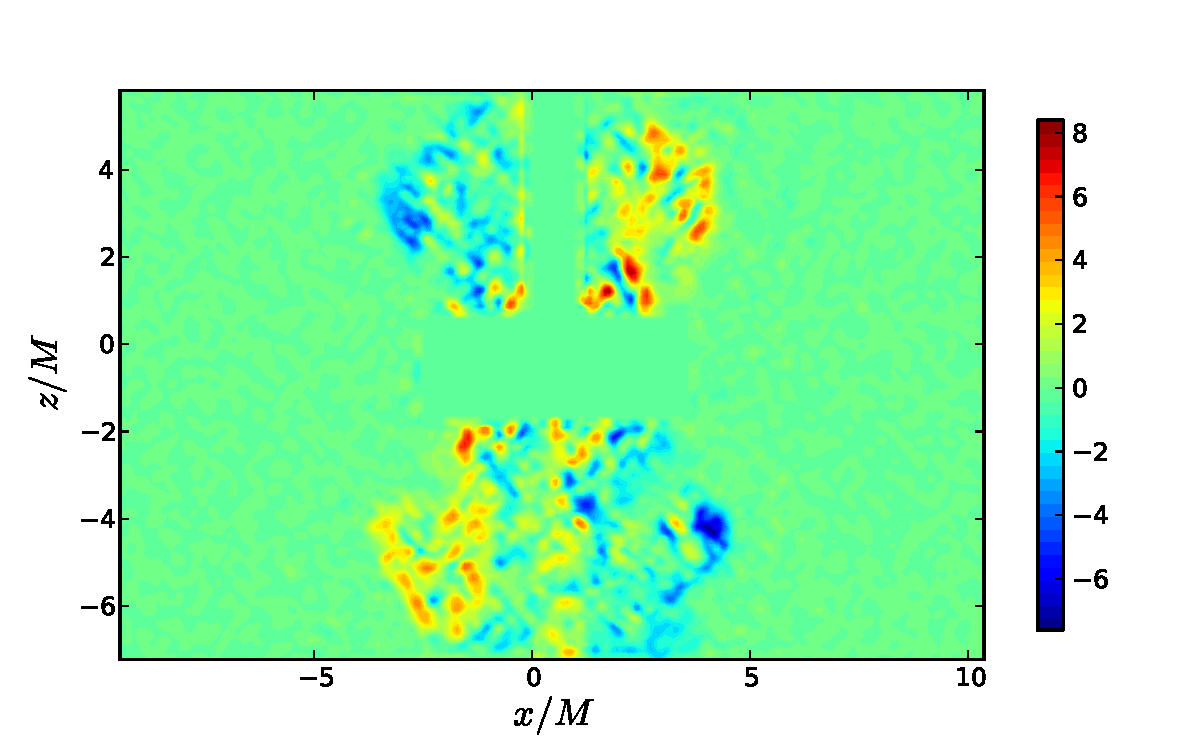
\includegraphics[width=0.4\textwidth]{figures/pivFreshDemo.pdf}
\caption{An instantaneous snapshot taken when the grid has just stopped oscillations at $t=8\unit{sec}$. Prior to this point the grid was oscillating with a frequency of $f=5\unit{Hz}$. Colour levels reflect the magnitude of $\omega_y$ computed from PIV data in units of $\unit{sec.^{-1}}$. \label{fig:pivFreshDemo}}
\end{figure}

Even though the turbulence continuously convects away from the grid, a boundary is formed between this convecting ``patch'' of turbulence and the quiescent surrounding fluid. In order to compare with the results from the experiments in stable stratification, it is desirable to algorithmically define the distance between the centre of the grid oscillations ($z=0$) and the average boundary between the turbulent/non-turbulent interface. The approach taken in the current study is similar to previous investigations \cite{Holzner2006,Krug2013}. A binary field is created by setting a threshold on the enstrophy ($\omega\cdot\omega$) field based on a percentage of the maximum enstrophy in the field. The furthest $z$ location of the detected turbulence from the grid is found for each horizontal location in the range $-2.5 \le x \le 2.5$, and these results are averaged to give a representative patch half-height. Furthermore, since the acquisition for the entire experimental set-up is triggered externally, the experiment could be repeated with a minimal amount of human-induced variation. Thus, in fresh water, each experiment was repeated 30 times, and the results in \figLabel\ref{fig:freshBoundaries} reflect the ensemble average of these 30 repetitions at each time step. The growth of the turbulence is observed to scale with the frequency; however, instead of scaling like $L_v\propto (kt)^{0.5}$ \cite{Long1978,Silva1994,Holzner2006} the initial growth scaled with $L_v=ft/4$ (also shown in \figLabel\ref{fig:freshBoundaries}). The observed plateau corresponds essentially with the edge of the PIV image plane.

\begin{figure}[ht]
\centering
\subfigure[]{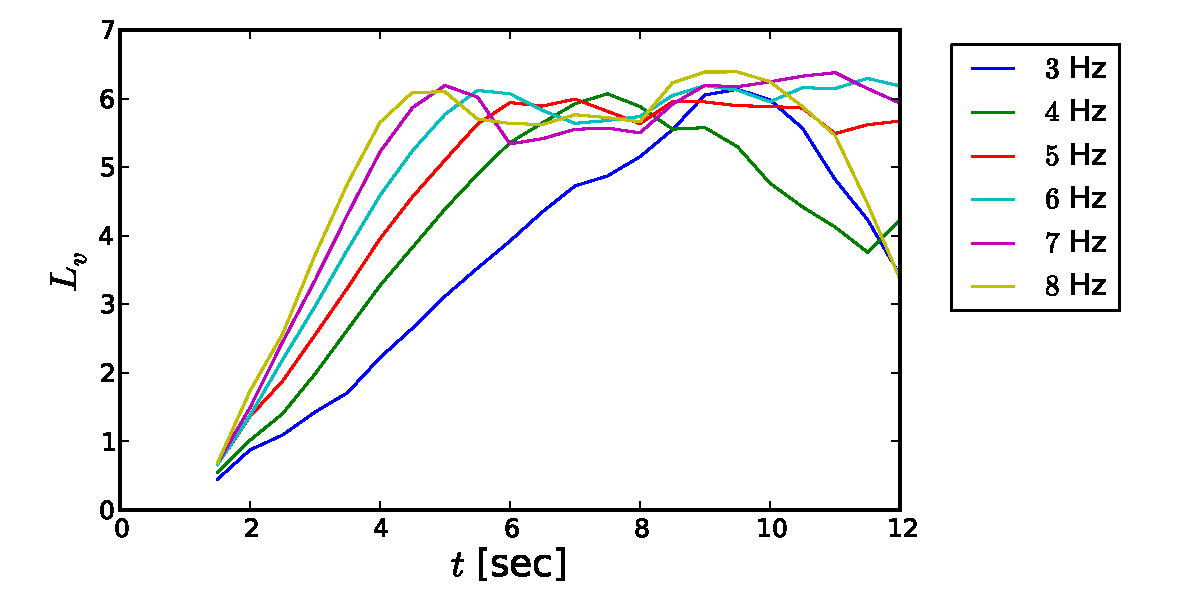
\includegraphics[width=0.5\textwidth]{figures/freshBoundary.pdf}}
\subfigure[]{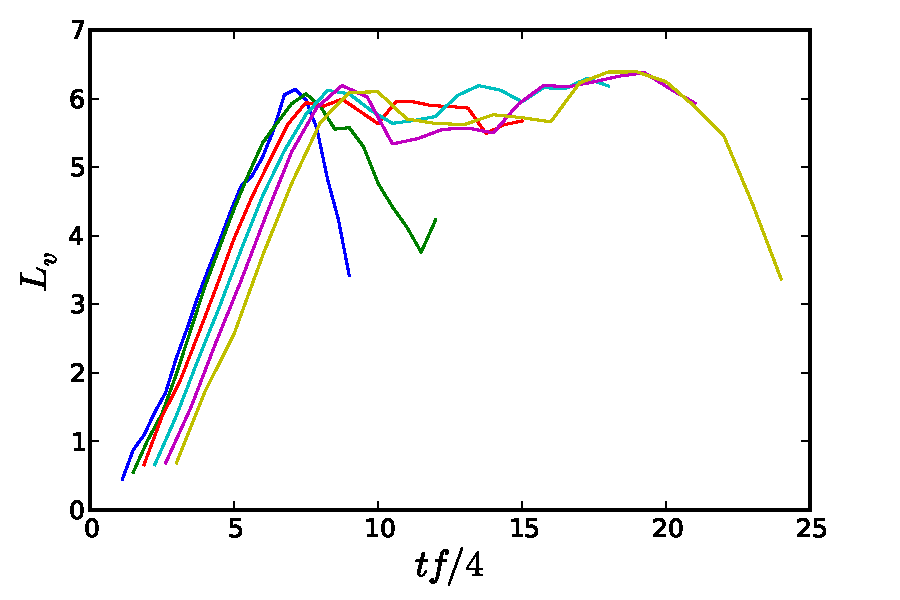
\includegraphics[width=0.35\textwidth]{figures/freshBoundaryScaled.pdf}}
\caption{Variation of the vertical height of the patch, $L_v$, with time $t$. The height is normalized using the mesh size, $M$. The patch height is determined from the enstrophy field based on an average of 30 samples for each time step and each frequency. The legend refers to the oscillation frequency of the grid.  In (b) the time axis is scaled based on the observed trends. \label{fig:freshBoundaries}}
\end{figure}

\subsection{Grid oscillations in a linear density gradient}
\label{sec:stratified_results}

The same range of frequencies used in the fresh water experiments was used for the experiments in stable stratification ($f=3-8\unit{Hz}$). As previously described, PLIF measurements were taken before the motion of the grid began to obtain the initial condition for each experiment. Density profiles at the non-dimensional time $Nt = 0$ are shown in \figLabel\ref{fig:rho_profile}. The amount of Rhodamine 6G decreases in the positive $z$-direction which increases the uncertainty in the estimate from the PLIF measurements. The choice was made to improve the resolution of the measurements beneath the grid since the grid-bearing bars also occur on the top of the grid, which obstruct the view. Nevertheless, the profile is observed to closely match a linear profile and provides the same initial condition for each experiment.

\begin{figure}[ht]
\centering
\subfigure[]{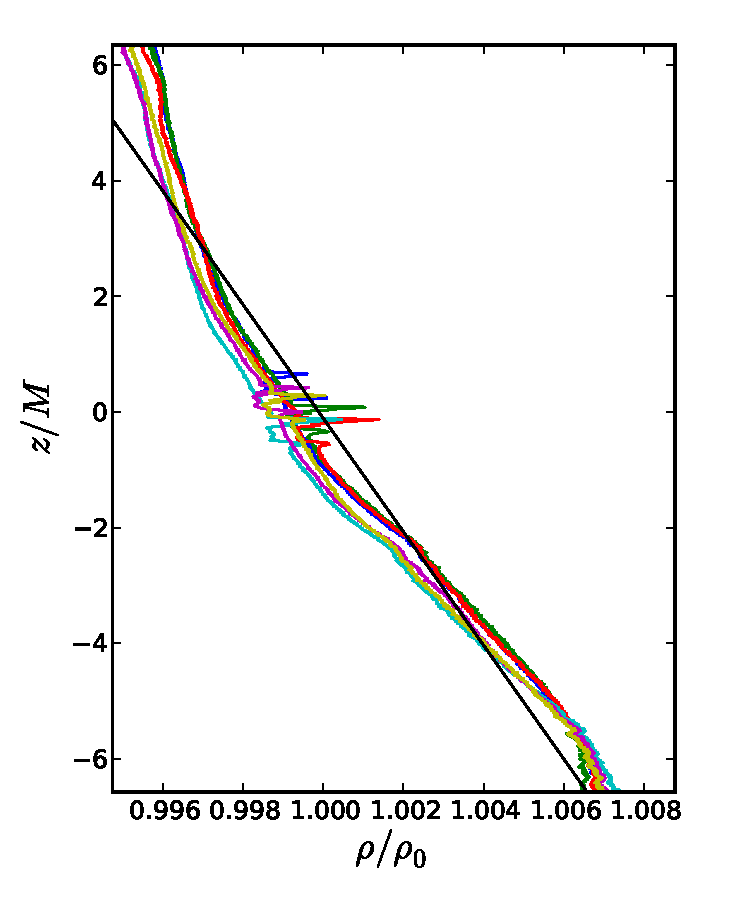
\includegraphics[height=5cm]{figures/index0_rho.pdf}}
\subfigure[]{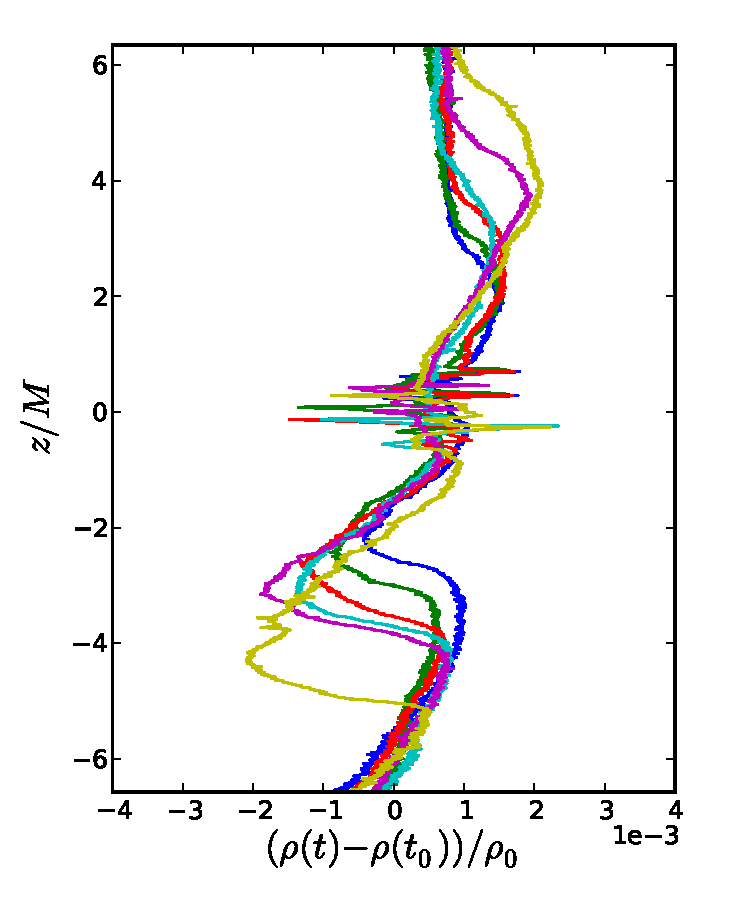
\includegraphics[height=5cm]{figures/index16_rho_fluc.pdf}}
\subfigure[]{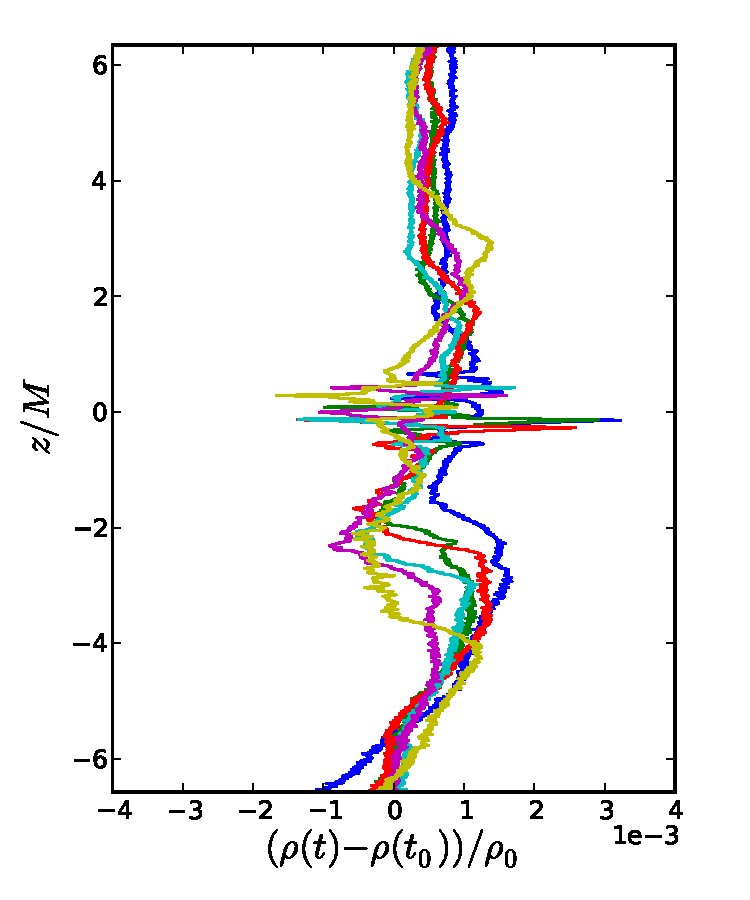
\includegraphics[height=5cm]{figures/index24_rho_fluc.pdf}}
\caption{Vertical density profiles taken at $x=1.4$ based from the PLIF measurements at three different non-dimensional times: (a) $Nt=0$, (b) $Nt=8$, and (c) $Nt = 12$. In each case the data are normalized by the reference density. In (b) and (c) the density fluctuations from $t=0$ are shown. \label{fig:rho_profile}}
\end{figure}

The life-cycle of the patch generated in the current study is partially demonstrated by the density profiles. After initiating oscillations at $Nt=0$, the patch is continuously fed energy until $Nt=8$, which is shown in \figLabel\ref{fig:rho_profile}(b). The presence of the grid in the imaging plane is observed near $z=0$ where significant density fluctuations are apparent. At $Nt=8$, \figLabel\ref{fig:rho_profile} demonstrates that the density begins to homogenize. This tendency towards near-uniform density distribution within the patch is suggested by previous experiments \cite{Silva1992,Silva1998} and the simplified model shown in \figLabel\ref{fig:thorpe}. However, it should be noted that in the current experiments the density does not become completely uniform as the mixing of the grid stops at $Nt=8$ and the patch collapses until the last snapshot $Nt=12$ and beyond.

\begin{figure}[h]
\centering
\subfigure[]{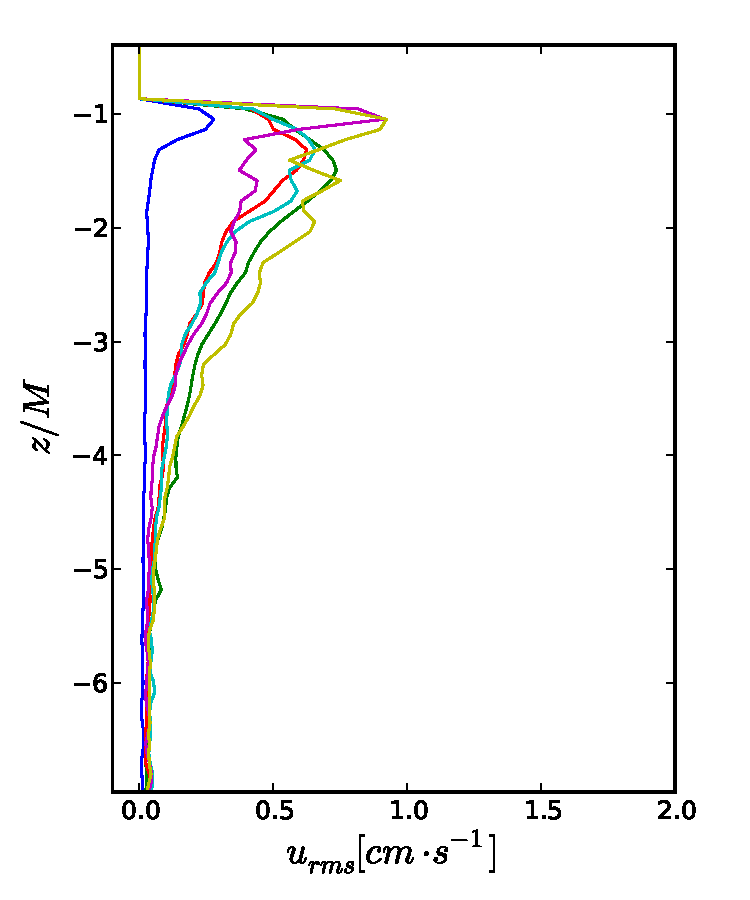
\includegraphics[height=5cm]{figures/index5_u.pdf}}
\subfigure[]{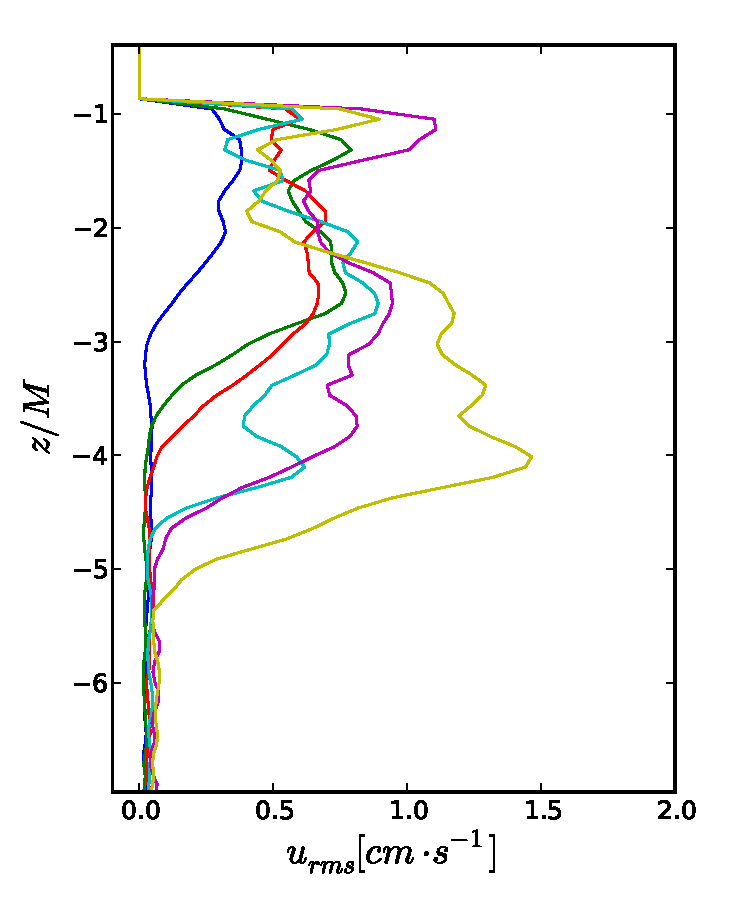
\includegraphics[height=5cm]{figures/index10_u.pdf}}
\subfigure[]{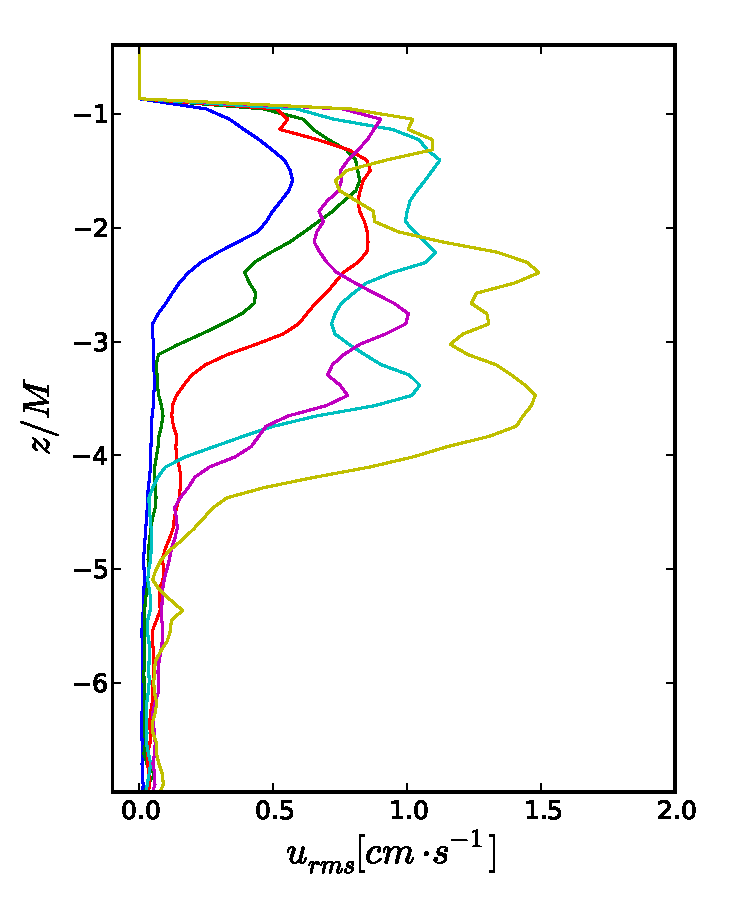
\includegraphics[height=5cm]{figures/index15_u.pdf}}
\subfigure[]{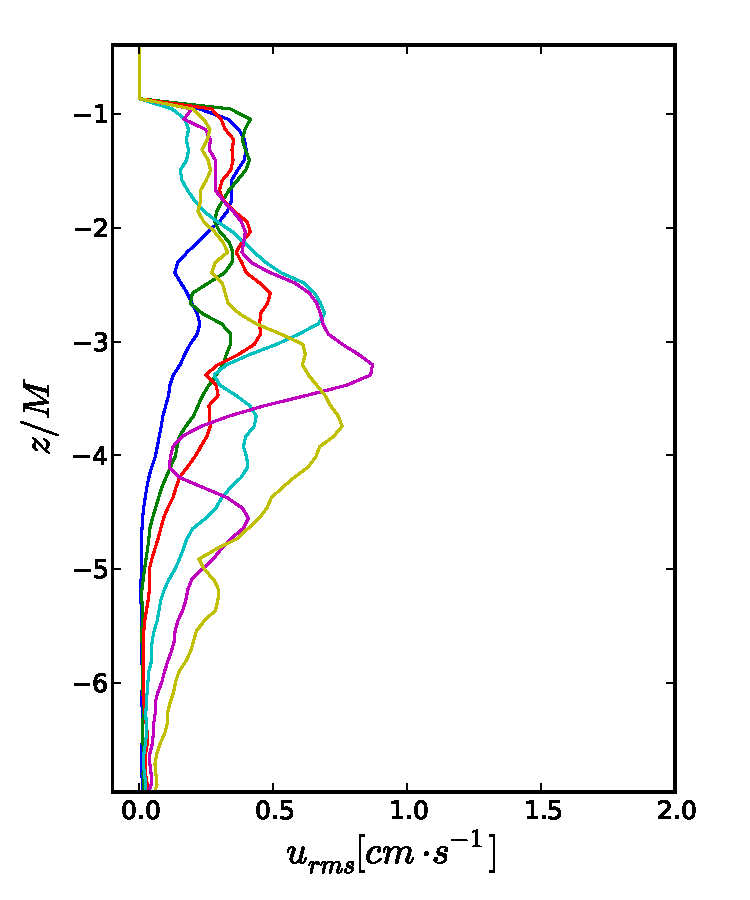
\includegraphics[height=5cm]{figures/index20_u.pdf}}
\caption{Instantaneous vertical profiles of $u_{rms}$ averaged between $-2.5 \le x \le 2.5$ from the PIV measurements at four different non-dimensional times: (a) $Nt=2.5$, (b) $Nt=5$, (c) $Nt = 7.5$, and (d) $Nt = 10$. The colouring of the lines matches the legend in \figLabel\ref{fig:rho_profile}. \label{fig:urms_profile}}
\end{figure}

\begin{figure}[h]
\centering
\subfigure[]{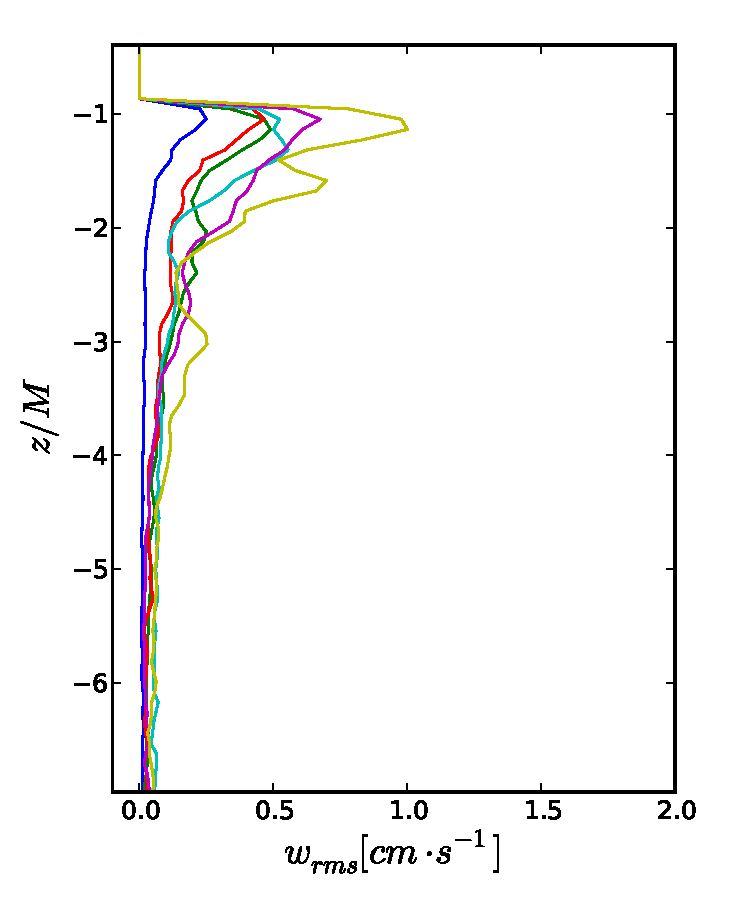
\includegraphics[height=5cm]{figures/index5_w.pdf}}
\subfigure[]{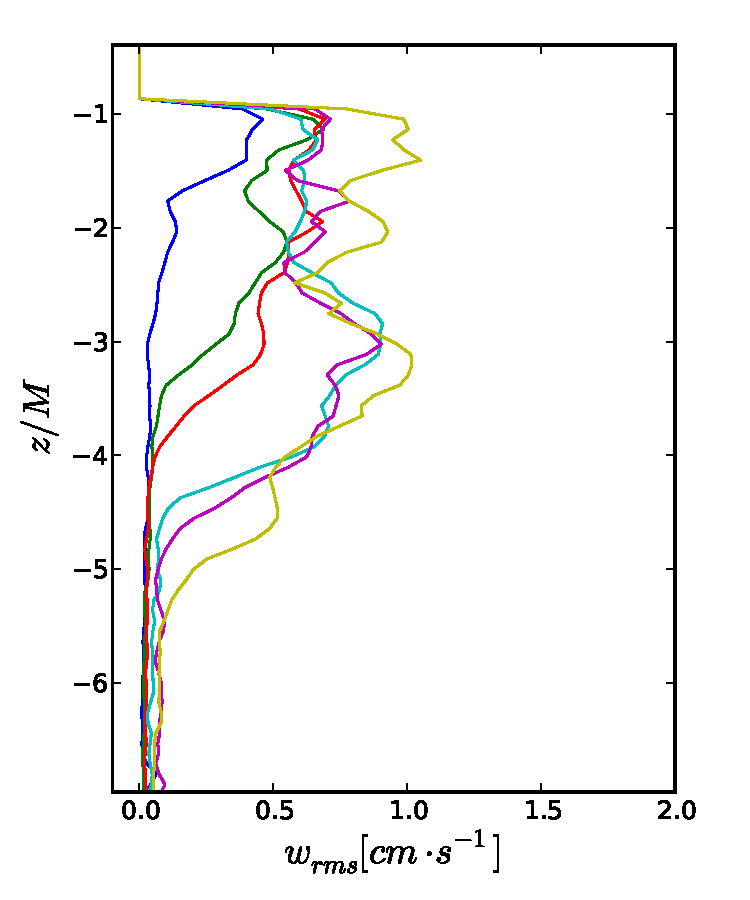
\includegraphics[height=5cm]{figures/index10_w.pdf}}
\subfigure[]{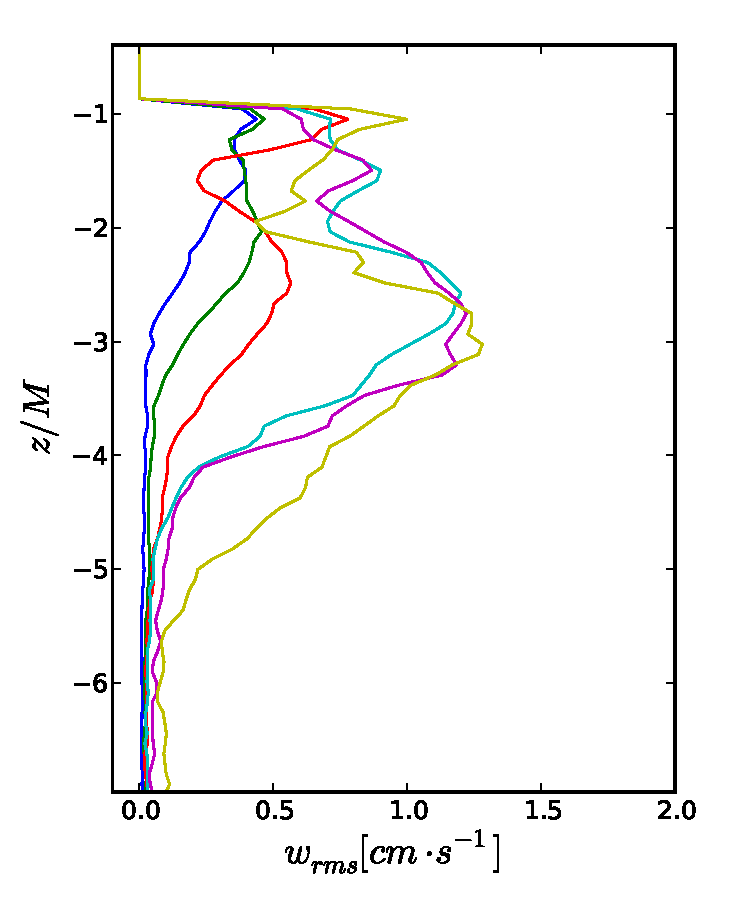
\includegraphics[height=5cm]{figures/index15_w.pdf}}
\subfigure[]{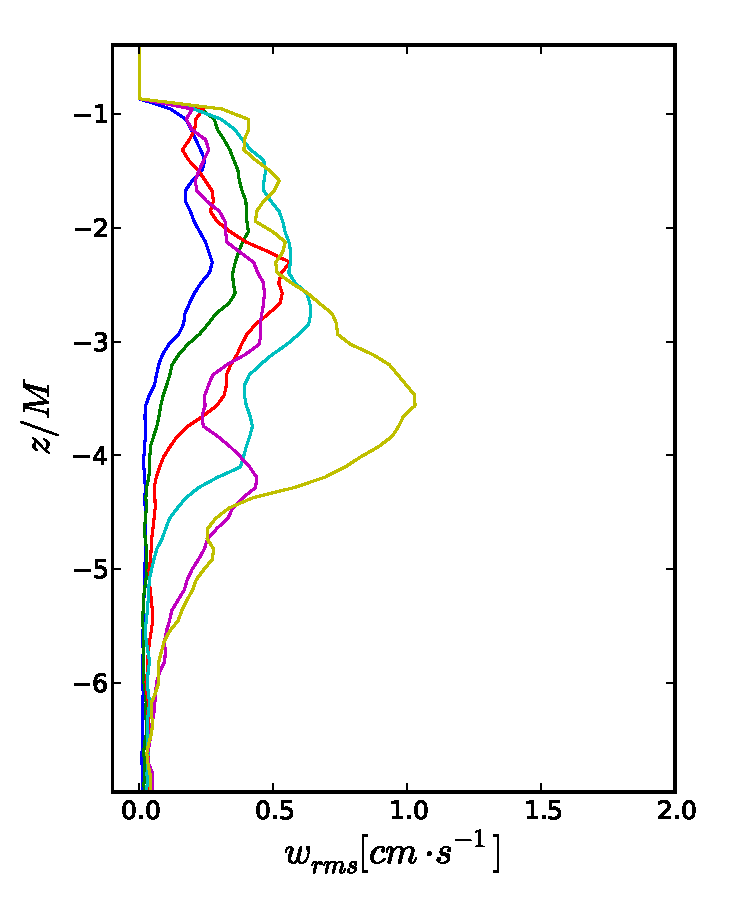
\includegraphics[height=5cm]{figures/index20_w.pdf}}
\caption{Instantaneous vertical profiles of $w_{rms}$ averaged between $-2.5 \le x \le 2.5$ from the PIV measurements at four different non-dimensional times: (a) $Nt=2.5$, (b) $Nt=5$, (c) $Nt = 7.5$, and (d) $Nt = 10$. The colouring of the lines matches the legend in \figLabel\ref{fig:rho_profile}. \label{fig:wrms_profile}}
\end{figure}

Turbulent velocity profiles are computed by assuming that a homogeneous region of the grid exists between $-2.5 \le x \le 2.5$ and averaging in the horizontal direction. The vertical profiles of $u_{rms}$ are calculated in this way and shown in \figLabel\ref{fig:urms_profile} with profiles of $w_{rms}$ shown in \figLabel\ref{fig:wrms_profile}. As expected, the magnitude of the velocity fluctuations increases with the frequency of the grid oscillation. In addition, high magnitudes of fluctuating velocity are observed at greater vertical distances from the grid as the frequency of the oscillations increases suggesting that the boundary of the patch also increases with the frequency of grid oscillations.

\begin{figure}[h]
\centering
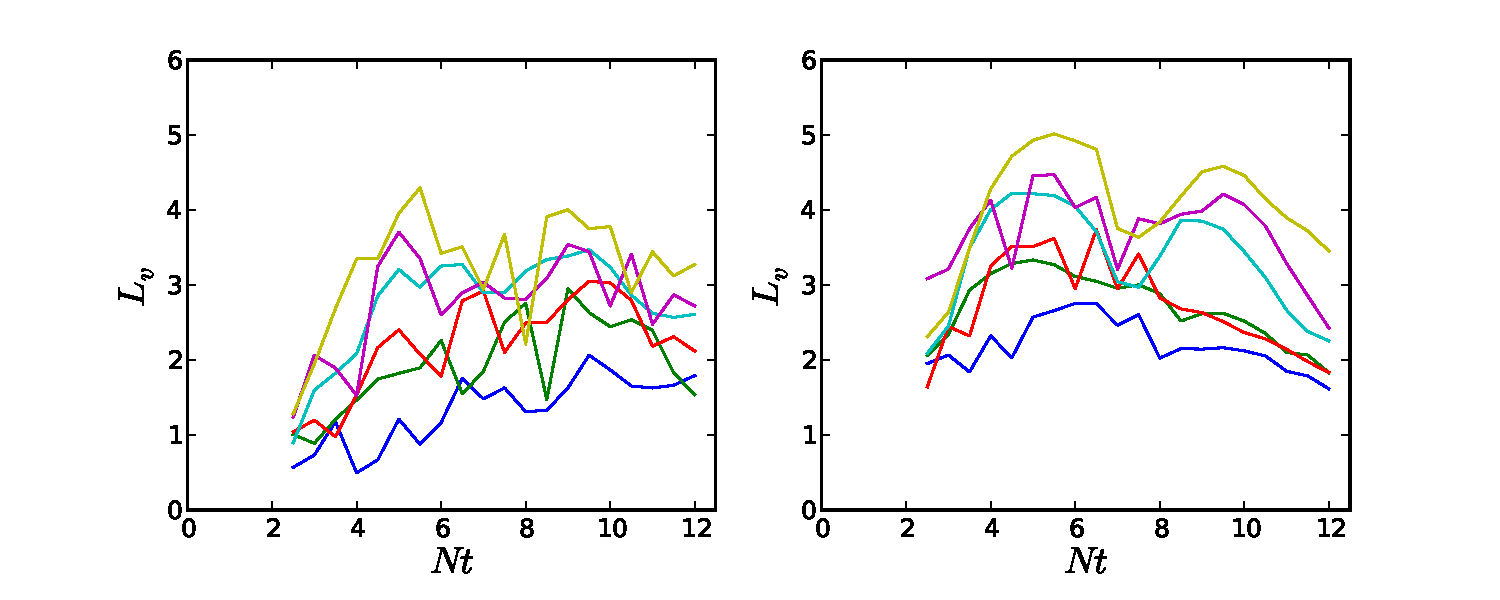
\includegraphics[width=0.7\textwidth]{figures/plifBoundaries.pdf}
\caption{Variation of the vertical height of the patch, $L_v$, with non-dimensional time $Nt$. The height is normalized using the mesh size, $M$. On the left, the patch height is determined from the enstrophy field, and on the right the patch height is determined using the density field. In each case the patch height is based on instantaneous samples.  \label{fig:plifBoundaries}}
\end{figure}

The patch boundaries have been determined for the experiments in stable stratification in the same way as described in the fresh water results. This method is based on using the enstrophy to mark the turbulent/non-turbulent interface. However, in the case of stable stratification there is also the need to consider the density interface. Previous experiments have not had sufficient spatial resolution to determine if the turbulent/non-turbulent interface also marks the density interface. Thus, in addition to defining the patch boundary by the enstrophy, the boundary is defined by the density gradient. The vertical patch height, $L_v$, is shown using both methods in \figLabel\ref{fig:plifBoundaries} where it is observed that the density boundary exceeds that determined by the enstrophy method. This observation implies that the vorticity field is attenuated as it approaches the sharp density interface. However, as is discussed in the next section, the vorticity generated is not necessarily limited to that within the patch.

The trends shown in \figLabel\ref{fig:plifBoundaries} generally agree with the comparable portion of the continuously forced experiments in \cite{Silva1998} where vertical growth of the patch was observed to halt at $Nt\approx4$. In the present set of experiments this is also observed to be the case regardless of the forcing frequency of the grid. However, the size of the patch is observed to vary considerably with the forcing frequency.

\section{DISCUSSION}

\begin{figure}[h]
\centering
\subfigure[]{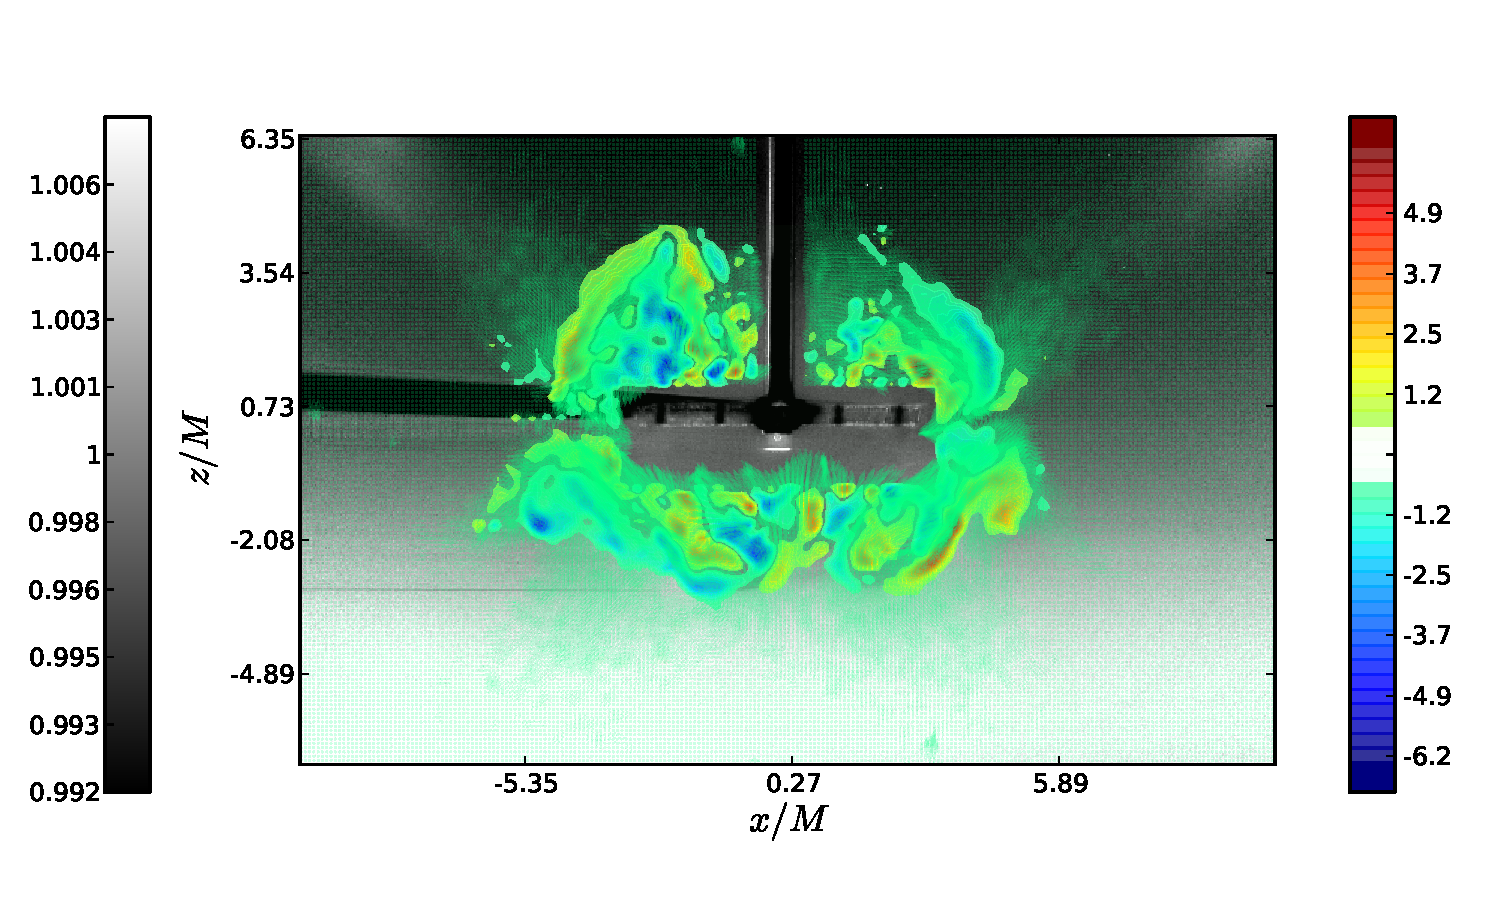
\includegraphics[width=0.55\textwidth]{figures/pivPlif_low_wide.pdf}}
\subfigure[]{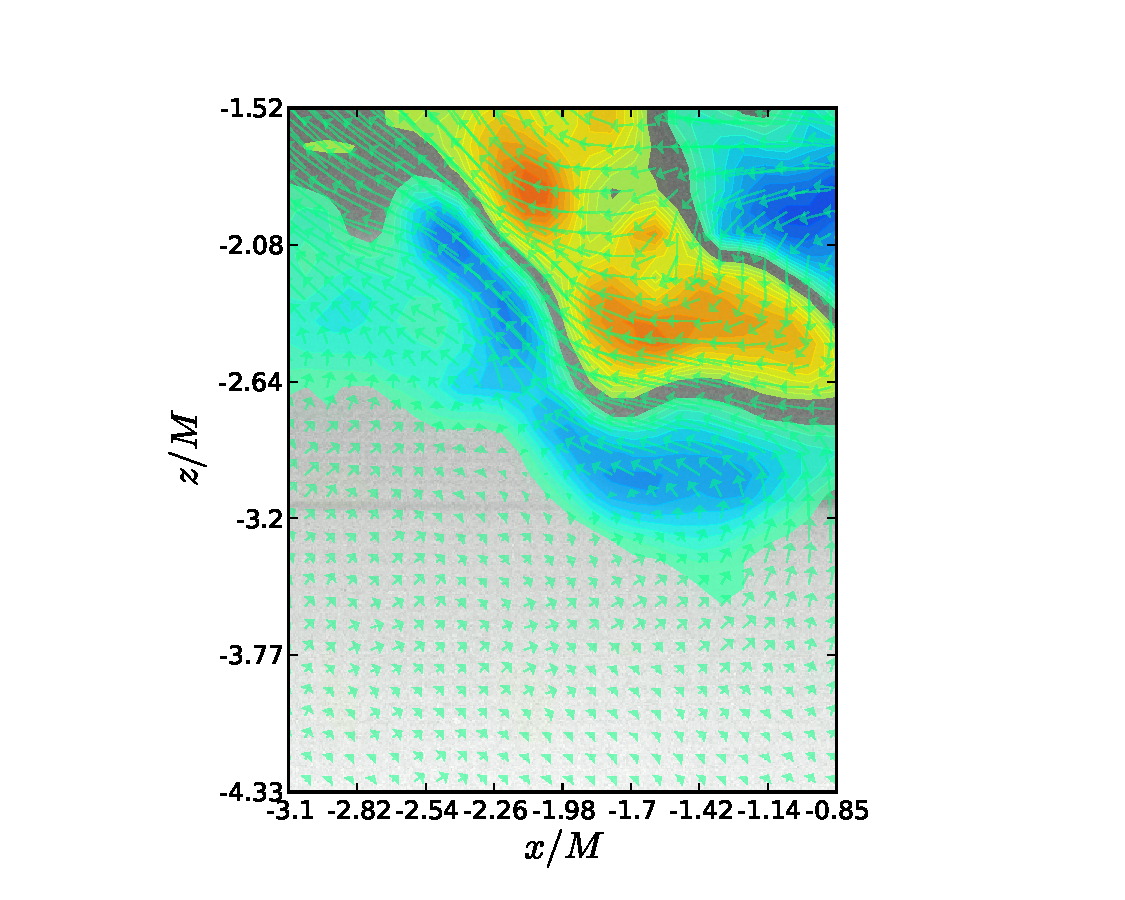
\includegraphics[width=0.35\textwidth]{figures/pivPlif_low_zoom.pdf}}
\caption{Instantaneous data taken at $Nt=8$ when the grid has just finished oscillating at $f=4\unit{Hz}$. The greyscale image represents the normalized density from the PLIF, the arrows represent the velocity from PIV, and the colours represent $\omega_y$ in units of $\unit{sec.^{-1}}$. In (b), a section is shown zoomed-in with the same colour scales and geometric scaling as (a). \label{fig:isoLow}}
\end{figure}

In the present set of experiments it is observed that the patch boundary, when defined by the density field, is distinct with a sharp gradient across the interface (i.e., \figLabel\ref{fig:isoLow}). As alluded to in the Introduction, diapycnal mixing (i.e., mixing across lines of constant density) is of considerable importance in oceanic turbulence. A clear example of its importance is the vorticity equation when density cannot be considered uniform
\begin{equation}
\frac{D\vect{\omega}}{Dt}=\vect{\omega}\cdot \nabla \vect{u} + \nu\nabla^2\vect{\omega} + \nabla p \times \nabla\left(\frac{1}{\rho}\right)
\end{equation}
where the last term (known as the baroclinic term) demonstrates how vorticity is generated whenever the pressure and density fields are not parallel \cite{bookTurner1973}. As indicated in \figLabel\ref{fig:thorpe}, the existence of the patch generates out-of-plane vorticity along its boundary due to the tilt of the isopycnal lines, and evidence of this vorticity at the patch boundary is present in \figLabel\ref{fig:isoLow} for grid oscillations of $f=4\unit{Hz}$.

\begin{figure}[h]
\centering
\subfigure[]{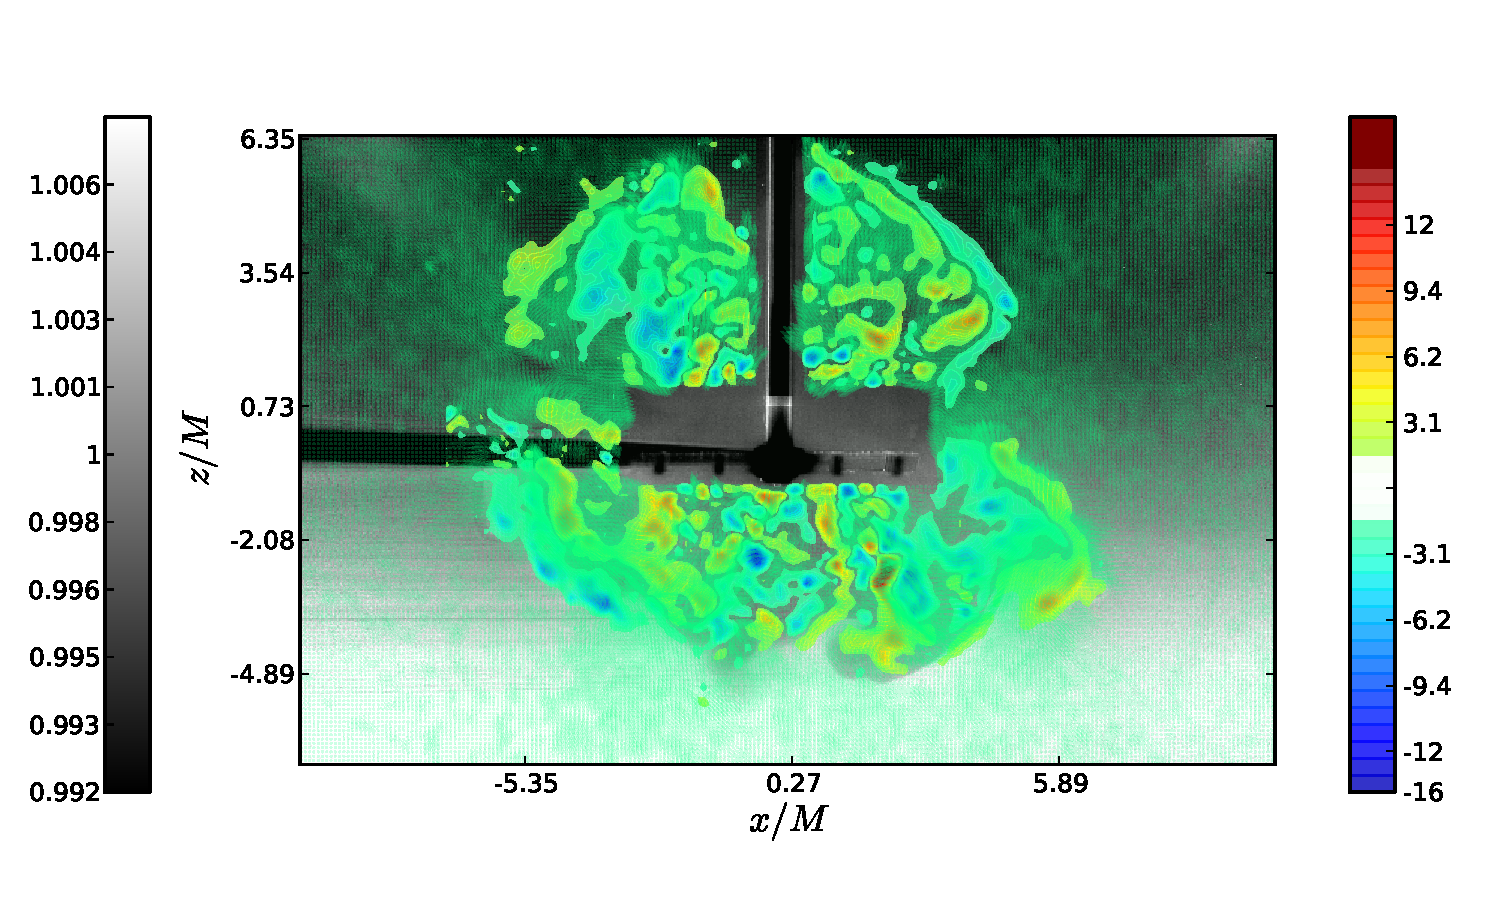
\includegraphics[width=0.55\textwidth]{figures/pivPlif_high_wide.pdf}}
\subfigure[]{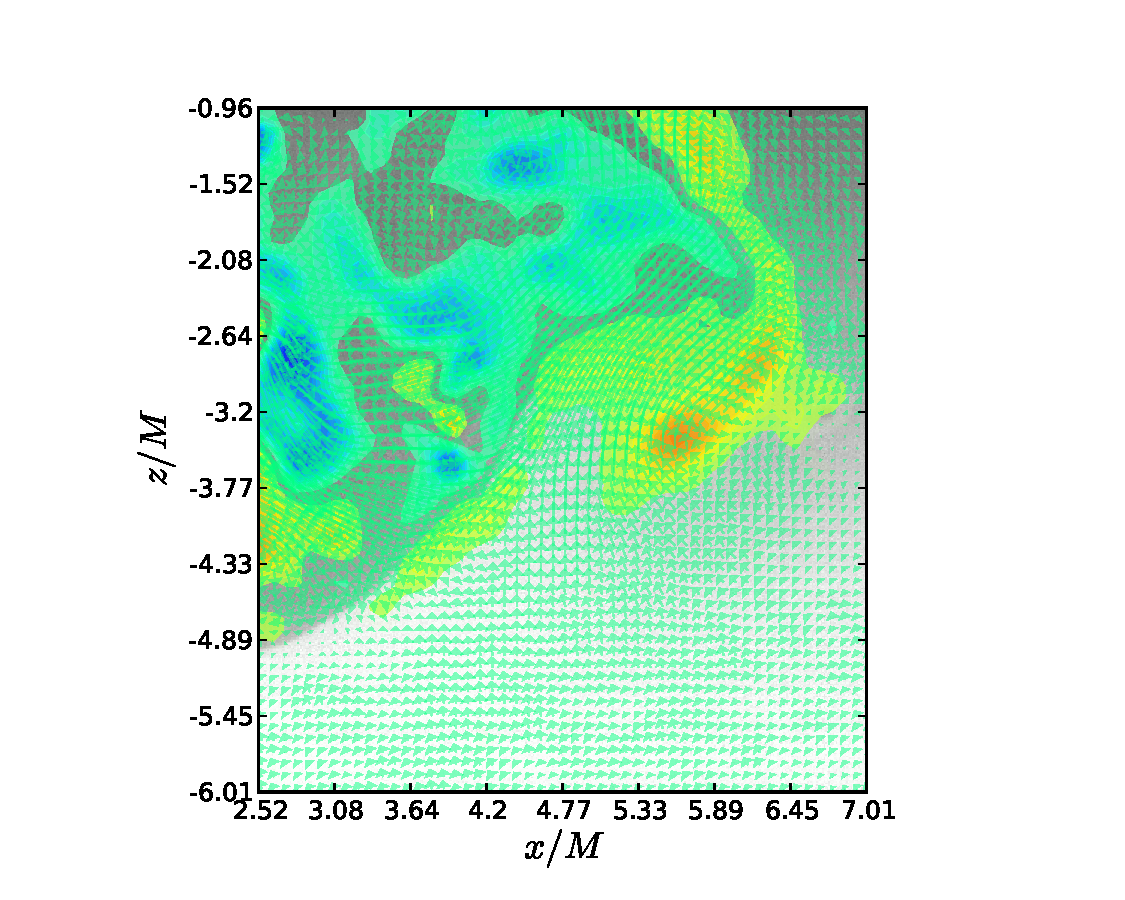
\includegraphics[width=0.35\textwidth]{figures/pivPlif_high_zoom.pdf}}
\caption{Instantaneous data taken at $Nt=8$ when the grid has just finished oscillating at $f=7\unit{Hz}$. The greyscale image represents the normalized density from the PLIF, the arrows represent the velocity from PIV, and the colours represent $\omega_y$ in units of $\unit{sec.^{-1}}$. In (b), a section is shown zoomed-in with the same colour scales and geometric scaling as (a). \label{fig:isoHigh}}
\end{figure}

When the grid oscillations are faster (shown in \figLabel\ref{fig:isoHigh} for $f=7\unit{Hz}$), the density interface is not observed to be as distinct - exemplified near $(x,z)=(6,-2.5)$. In these experiments, the grid is of finite extent and it generates strong vortices at its horizontal edges. This tendency is shown schematically in \figLabel\ref{fig:exp_schematic} and in the data (e.g., \figLabel\ref{fig:pivFreshDemo}). The generated vortices have the opposite vorticity than that generated at the patch boundary and grow stronger with increased oscillation frequency. Therefore, the mixing at the boundary of the patch intensifies and the patch boundary becomes more diffuse (\figLabel\ref{fig:isoHigh}) as the grid-generated vorticity interacts with the baroclinic vorticity.

\FloatBarrier
\section{CONCLUSION}

An experimental method has been developed to simultaneously sample velocity and density data with high spatial resolution in a fluid with stable stratification. In order to achieve reliable results, it was necessary to achieve stratification using two solutions which have the same index-of-refraction both separately and when mixed. In the current experiments, the heavy liquid was a solution of water and Epsom salts while the lighter liquid was formed using water and sugar. In order to measure the density field, Rhodamine 6G was added to the heavy liquid and PLIF measurements were performed. These PLIF measurements were synchronized with PIV thus ensuring simultaneous capture of the velocity and density fields.

The growth of the turbulent patch in fresh water was observed to be largely unbounded. The turbulent/non-turbulent interface was identified using the enstrophy field and the distance of this interface increased monotonically from the grid with time. The same height was computed in the case of stable stratification in addition to the patch height as defined by the density interface. It was shown that the density interface was farther from the grid than the turbulent/non-turbulent interface. However, it was observed that vorticity was present at horizontal locations outside of the density-defined patch boundaries.

The baroclinic term in the vorticity equation, coupled with a sharp density interface, predicts the occurrence of vorticity along the isopycnals at the patch boundary. This vorticity was observed along the patch boundary in each case. However, as the frequency of the grid oscillations increased, the density interface at the patch boundary was observed to be more diffuse. 

\section*{ACKNOWLEDGEMENTS}

Z.J. Taylor is grateful to the Azrieli Foundation for the award of an Azrieli Fellowship. The authors acknowledge support of the  Bi-National U.S.-Israel Science Foundation Grant No. 2008051. For help during the experiments, the authors also wish to thank Mark Baevsky and Lilly Verso.

%\bibliographystyle{unsrt}
%\bibliography{../../../research_papers/paperdb,../../../books/booklist}
\input{bib.bbl}

\end{document}
